\usetikzlibrary{calc}
\usetikzlibrary{positioning}
\usetikzlibrary{shapes}
\usetikzlibrary{intersections,decorations.markings}
\usetikzlibrary{arrows.meta}
\usetikzlibrary{fit}
\usetikzlibrary{automata}

%\usepackage{../includes/nick-shorthands}

\newcommand{\lblTextsize}{\small}

%% COMMANDS %%

\newcommand{\textoverline}[1]{{$\overline{\mbox{#1}}$}}
\newcommand{\textinmath}[1]{\textnormal{\scriptsize{#1}}}

\newcommand{\pathdots}[2]{\path (#1) -- node[pos=0.54,sloped,font=\Huge]{\dots} (#2);}

\newcommand{\arrow}[2]{\draw [-latex] (#1) -- (#2);}
\newcommand{\arrowlbl}[4][]{\draw [-latex] (#2) -- node[#1]{#4} (#3);}
\newcommand{\edgearcarrowlbl}[5][]{\draw [-latex] (#2) -- ++(#4) -- node[#1]{#5} ($(#3)+(#4)$) -- (#3);}

%\newcommand{\algoloop}[1][2][{\node at ($(+#1.west)+(-0.5,+0.5)$) {frontend};
%	\draw [-latex, thick, rounded corners] ($(transmit.north west)+(+0.2,+0.2)$) -| ($(transmit.south east)+(+0.2,-0.2)$) -- ($(transmit.south west)+(-0.2,-0.2)$) |- ($(transmit.north west)+(+0.2,+0.2)$);


%% GENERIC %%

\usetikzlibrary{calc}

\tikzset{
	%
	box/.pic={
		\node [ draw, rectangle, minimum width=1.2cm, minimum height=1.2cm ] at (0,0) (-box) {};
	},
	myellipse/.pic={
		\node [ draw, ellipse, minimum width=2cm, minimum height=1cm ] at (0,0) (-box) {};
	}
	%
}
\tikzset{
%
greenbox/.pic={
	\node [ draw=green, very thick, rectangle, minimum width=1.2cm, minimum height=1.2cm ] at (0,0) (-box) {};
}
%
}

\tikzset{
	%
	shuffle-arrows/.pic={
		\begin{scope}[scale=0.6,shift={(-0.5,-0.25)}]
			\draw[->, thick, line cap=round] (0.0,0.5) .. controls (0.5,0.5) and (0.5,0.0) .. (1.0,0.0);
			\draw[line width=2.5pt, white] (0.0,0.0) .. controls (0.5,0.0) and (0.5,0.5) .. (1.0,0.5);
			\draw[->, thick, line cap=round] (0.0,0.0) .. controls (0.5,0.0) and (0.5,0.5) .. (1.0,0.5);
		\end{scope}
	}
	%
}

\tikzset{
	%
	pics/constellation/.style args={#1}{
		code={
			\draw[#1, line cap=round] (-0.33,0) -- (0.33,0);
			\draw[#1, line cap=round] (0,0.33) -- (0,-0.33);
			\draw[#1, fill=#1] (-0.15,-0.15) circle (0.04);
			\draw[#1, fill=#1] (0.15,-0.15) circle (0.04);
			\draw[#1, fill=#1] (-0.15,0.15) circle (0.04);
			\draw[#1, fill=#1] (0.15,0.15) circle (0.04);
			\draw [#1] (0,0) circle (0.212);
		}
	}
	%
}

\tikzset{
	%
	wave/.pic={
		\begin{scope}[scale=0.7, shift={(-0.6,-0.35)}]
			\begin{axis}[
				xmin=-70, xmax=790, 
				ymin=-1.1, ymax=1.1,
				hide x axis,
				hide y axis,
				width=8em,
				height=6.5em
			]
				\addplot [domain=0:720, samples=100, thick, line cap=round] {sin(x)};
			\end{axis}
		\end{scope}
	}
	%
}

\tikzset{
	%
	pics/smallwave/.style args={#1}{
		code={
		\begin{scope}[scale=0.7, shift={(-0.6,-0.35)}]
			\begin{axis}[
				xmin=-0.1, xmax=4.1, 
				ymin=-1.1, ymax=1.1,
				hide x axis,
				hide y axis,
				width=8em,
				height=6.5em,
				color=#1
			]
				\addplot [domain=0:4, samples=100, thick, line cap=round] {0.4*sin(x*360)};
			\end{axis}
		\end{scope}
	}
},
pics/smallwave/.default=black
}


\tikzset{
%
pics/shortwave/.style args={#1}{
	code={
	\begin{scope}[scale=0.7, shift={(-0.6,-0.35)}]
		\begin{axis}[
			xmin=-0.1, xmax=1.9, 
			ymin=-1.1, ymax=1.1,
			hide x axis,
			hide y axis,
			width=5.5em,
			height=6.5em,
			color=#1
			]
			\addplot [domain=0:4, samples=100, thick, line cap=round] {0.4*sin(x*360)};
		\end{axis}
	\end{scope}
	}
},
pics/shortwave/.default=black
}

\tikzset{
	%
	pics/sinc/.style args={#1}{
		code={
		\begin{scope}[scale=0.7, shift={(-0.6,-0.35)}]
			\begin{axis}[
				xmin=-700, xmax=700, 
				ymin=-0.5, ymax=2.1,
				hide x axis,
				hide y axis,
				width=8em,
				height=6.5em,
				color=#1
			]
				\addplot [domain=-680:680, samples=200, thick, line cap=round] {sin(x)/(x/360*3.14)};
			\end{axis}
		\end{scope}
	}
},
pics/sinc/.default=black
}

\tikzset{
%
cp_cs/.pic={
	\begin{scope}[scale=0.7, shift={(-0.6,-0.35)}]
		\begin{axis}[
			xmin=-700, xmax=700, 
			ymin=-2, ymax=2,
			hide x axis,
			hide y axis,
			width=8em,
			height=6.5em
			]
			\addplot [domain=-680:680, samples=200, thick, line cap=round] {cos(x)};
		\end{axis}
	\end{scope}
}
}

\tikzset{
	%
	whitebox/.pic={
		\node [ draw, rectangle, fill=white, minimum width=.05cm, minimum height=.5cm ] at (0,0) (-box) {};
	}
	%
}



\tikzset{
	%
	pics/rnd1/.style args={#1}{
		code={
		\begin{scope}[scale=0.7, shift={(-0.6,-0.35)}]
			\begin{axis}[
				xmin=-700, xmax=700, 
				ymin=-5, ymax=5,
				hide x axis,
				hide y axis,
				width=7em,
				height=6.5em,
				color=#1
				]
				\addplot [domain=-680:680, samples=200, thick, line cap=round] {sin(x)-3};
				\addplot [domain=-680:680, samples=200, thick, line cap=round] {cos(x)};
				\addplot [domain=-680:680, samples=200, thick, line cap=round] {sin(x)+3};
			\end{axis}
		\end{scope}
	}
},
pics/rnd1/.default=black
}

\tikzset{
	%
	die/.pic={
		\draw (-0.3,-0.3) rectangle (0.3,0.3);
	}
	%
}

\tikzset{
	%
	magnifier/.pic={
		\draw[thick, line cap=round, inner sep=0] (0,0) circle (0.14);
		\draw[very thick, line cap=round, inner sep=0] (0.11,-0.11) -- (0.22,-0.22);
	}
	%
}

\tikzset{
	%
	ruler/.pic={
		\begin{scope}[scale=0.045]
			\draw (-10,2) rectangle (10,-2);
			\foreach \x in {-9,-6,...,9} {%
				\draw (\x,2) -- (\x,0.2);
				\ifnum \x<9
					\foreach \y in {1,2} {%
						\draw ($(\x,2)+(\y,0)$) -- ($(\x,1)+(\y,0)$);
					};
				\fi
			};
		\end{scope}
	}
	%
}



%% COMPONENTS %%

\tikzset{
	interleaver/.pic={
		\pic[shift={(0,-0.2)}]{shuffle-arrows};
		\node at (0.00,0.3) {\textsf{Intv}};
		\pic {box};
	}
}

\tikzset{
	deinterleaver/.pic={
		\pic[shift={(0,-0.2)}]{shuffle-arrows};
		\node at (0.00,0.3) {\textsf{De-Intv}};
		\pic {box};
	}
}

\tikzset{
	enc-nsnr/.pic={
		\node at (0.0, 0.35) {\textsf{\small{Cv-Enc}}};
		\node at (0.0,-0.02) {\textsf{\large{\textoverline{S}-\textoverline{R}}}};
		\node at (0.0,-0.42) {\textsf{\footnotesize{1/2}}};
		\pic {box};
	}
}

\tikzset{
	enc-sr-acc/.pic={
		\node at (0.0, 0.35) {\textsf{\small{Cv-Enc}}};
		\node at (0.0,-0.02) {\textsf{\large{S-R}}};
		\node at (0.0,-0.38) {\textsf{\footnotesize{ACC}}};
		\pic {box};
	}
}

\tikzset{
	dec-nsnr/.pic={
		\node at (0.0, 0.35) {\textsf{\small{Cv-Dec}}};
		\node at (0.0,-0.02) {\textsf{\large{\textoverline{S}-\textoverline{R}}}};
		\node at (0.0,-0.42) {\textsf{\footnotesize{1/2}}};
		\pic {box};
	}
}

\tikzset{
	dec-sr-acc/.pic={
		\node at (0.0, 0.35) {\textsf{\small{Cv-Dec}}};
		\node at (0.0,-0.02) {\textsf{\large{S-R}}};
		\node at (0.0,-0.38) {\textsf{\footnotesize{ACC}}};
		\pic {box};
	}
}

\tikzset{
	encoder/.pic={
		\node at (0,-0.18) {%
			\footnotesize{$\overline{\underline{1010}}$}%
			\hspace{0.4ex}%
			\footnotesize{$\overline{\underline{11}}$}%
		};
		\node at (0.00,0.34) {\textsf{\small{Encod}}};
		\pic {box};
	}
}

\tikzset{
	pics/decoder/.style args={#1}{
		code={
			\node [#1] at (0,-0.18) {%
				\footnotesize{$\overline{\underline{1010}}$}%
				\hspace{0.4ex}%
				\footnotesize{$\overline{\underline{11}}$}%
			};
			\node [#1] at (0.00,0.34) {\textsf{\small{Decod}}};
		}
	},
	pics/decoder/.default=black
}

\tikzset{
	mapper/.pic={
		\pic[shift={(0,-0.18)}]{constellation};
		\node at (0.00,0.31) {\textsf{\small{Map}}};
		\pic {box};
	}
}

\tikzset{
	pics/demapper/.style args={#1}{
		code={
			\pic[shift={(0,-0.18)}]{constellation=#1};
			\node [#1] at (0.00,0.31) {\textsf{\small{Demap}}};
		}
	},
	pics/demapper/.default=black
}



\tikzset{
	resource_mapper/.pic={
		\pic[shift={(-0.08,-0.18)}]{shortwave};
		\pic[shift={(0.25,-0.18)}]{rnd1};
		\node at (0.00,0.34) {\textsf{\small{S/P}}};
		\pic {box};
	}
}

\tikzset{
	resource_mapper/.pic={
		\pic[shift={(-0.08,-0.18)}]{shortwave};
		\pic[shift={(0.25,-0.18)}]{rnd1};
		\node at (0.00,0.34) {\textsf{\small{S/P}}};
		\pic {box};
	}
}

\tikzset{
	pics/fft/.style args={#1}{
		code={
		\pic[shift={(-0.08,-0.18)}]{shortwave=#1};
		\pic[shift={(0.25,-0.18)}]{rnd1=#1};
		\node [#1] at (0.00,0.34) {\textsf{\small{FFT}}};
		}
	}
}

\tikzset{
	pics/idft/.style args={#1}{
		code={
		\pic[shift={(-0.08,-0.18)}]{rnd1=#1};
		\pic[shift={(0.6,-0.18)}]{shortwave=#1};
		\node [#1] at (0.00,0.34) {\textsf{\small{IDFT}}};
		}
	}
}



\tikzset{
	cp/.pic={
		\pic[shift={(0,-0.18)}]{cp_cs};
		\pic[shift={(-0.12,-0.17)}, scale=0.95, white] {whitebox};
		\node at (0.00,0.34) {\textsf{\small{CP/CS}}};
		\pic {box};
	}
}


\tikzset{
	modulator/.pic={
		\pic[shift={(0,-0.18)}]{sinc};
		\node at (0.00,0.34) {\textsf{\small{Mod}}};
		\pic {greenbox};
	}
}

\tikzset{
	demodulator/.pic={
		\pic[shift={(0,-0.18)}]{sinc};
		\node at (0.00,0.34) {\textsf{\small{Demod}}};
		\pic {greenbox};
	}
}

\tikzset{
	equalizer/.pic={
		\pic[shift={(0,-0.18)}]{sinc};
		\node at (0.00,0.34) {\textsf{\small{Inv}}};
	}
}

\tikzset{
	detector/.pic={
		\pic[shift={(0,-0.18)}] {smallwave};
		\pic[shift={(0,-0.17)}, scale=0.95, white] {magnifier};
		\pic[shift={(0,-0.17)}, scale=1.27, white] {magnifier};
		\pic[shift={(0,-0.17)}, scale=1.1] {magnifier};
		\node at (0.00,0.34) {\textsf{\small{Detect}}};
		\pic {box};
	}
}
\tikzset{
	synchronizer/.pic={
		\pic[shift={(0,-0.18)}] {smallwave};
		\pic[shift={(0,-0.17)}, scale=0.95, white] {magnifier};
		\pic[shift={(0,-0.17)}, scale=1.27, white] {magnifier};
		\pic[shift={(0,-0.17)}, scale=1.1] {magnifier};
		\node at (0.00,0.31) {\textsf{\small{Sync}}};
	}
}

\tikzset{
	estimator/.pic={
		\pic[shift={(0,-0.14)}, scale=0.55] {constellation};
		\draw[white, fill=white] (-0.4,-0.24) rectangle (0.4,-0.5);
		\pic[shift={(0,-0.33)}, scale=0.8] {ruler};
		\node at (0.00,0.34) {\textsf{\small{Estim}}};
	}
}

\tikzset{
	source/.pic={
		\node at (0,0.34) {\textsf{\small{Source}}};
		\node at (0,-0.18) {\small{$\overline{\underline{1010}}$}};
		\pic {box};
	}
}

\tikzset{
	data/.pic={
		\node at (0,0.34) {\textsf{\small{Data}}};
		\node at (0,-0.18) {\small{$\overline{\underline{1010}}$}};
		\pic {box};
	}
}

\tikzset{
	rayleigh/.pic={
		\begin{scope}[shift={(-0.43,-0.16)}]
			\begin{axis}
				[ width=69.5pt, height=62pt, axis x line=bottom, outer axis line style={-}, xtick=\empty, ytick=\empty ]
				\addplot [samples=200] { 1/sqrt(1-x^2) };
			\end{axis}
		\end{scope}
		\node at (0,-0.4) {\textsf{\scriptsize{Rayleigh}}};
		\pic {box};
	}
}

\tikzset{
	white-gaussian/.pic={
		\begin{scope}[shift={(-0.43,-0.16)}]
			\begin{axis}
				[ width=69.5pt, height=62pt, axis x line=bottom, outer axis line style={-}, xtick=\empty, ytick=\empty ]
				\addplot [samples=200] { 1/sqrt(6*3^2) * exp( -x^2 / sqrt(6*3^2) ) };
			\end{axis}
		\end{scope}
		\node at (0,-0.4) {\textsf{\scriptsize{Gauss}}};
		\pic {box};
	}
}

\tikzset{
	hard-decision/.pic={
		\node at (0,0.28) {\textsf{\small{Hard}}};
		\draw[thick,shift={(0,-0.2)}] (-0.2,-0.2) -- (0,-0.2) -- (0,0.2) -- (0.2,0.2);
		\pic {box};
	}
}

\tikzset{
	add/.pic={
		\draw [ line cap=round ] (-0.2,0) -- (0.2,0);
		\draw [ line cap=round ] (0,-0.2) -- (0,0.2);
		\draw (0,0) circle (0.25);
		\node [ minimum width=0.5cm, minimum height=0.5cm ] at (0,0) (-box) {};
	}
}

\tikzset{
	multiply/.pic={
		\draw [ line cap=round ] (-0.141,-0.141) -- (+0.141,+0.141);
		\draw [ line cap=round ] (-0.141,+0.141) -- (+0.141,-0.141);
		\draw (0,0) circle (0.25);
		\node [ minimum width=0.5cm, minimum height=0.5cm ] at (0,0) (-box) {};
	}
}
\tikzset{
	blub/.style args={#1}{draw=#1, inner sep=0, ellipse, fill=white, minimum width=1.2cm, minimum height=0.5cm},
	copy/.style={blub, color=gray!80},
	pics/antenna/.style args={#1}{
		code={
			\draw [color=#1] (0,0) -- (50:0.5);
			\draw [color=#1] (0,0) -- (130:0.5);
			\draw [color=#1] (0,0) -- (0,-0.5);
		}
	},
	pics/frontend/.style args={#1}{
		code={
			\node[inner sep=0] (-ant) {
				\tikz[xshift=2cm]{ 
					\pic [anchor=west] at (0,0) {antenna=#1};
				}
			};	
%			\pic (-ant) at (0,0) {antenna=#1};
			
			\node[blub=#1, right= of -ant] (-b) {
				\tikz{ 
					\pic [anchor=center]{synchronizer};
				}
			};
			\node[blub=#1, right= of -b] (-c) {
				\tikz{ 
					\pic [anchor=center] at (0,0) {fft=#1};
				}
			};
			\node[blub=gray!80, below= of -c] (-d) {
				\tikz{ 
					\pic [anchor=center] at (0,0) {fft=gray!80};
				}
			};
			\node[blub=#1, right= of -c] (-e) {
				\tikz{ 
					\pic [anchor=center] at (0,0) {estimator};
				}
			};

			\draw [-Stealth, color=#1] (-ant) -- (-b);
			\draw [-Stealth, color=#1, name path=-t] (-b) -- (-c);
			\draw [-Stealth, dashed, color=gray!80] (-b) -- (-d);	
			\draw [-Stealth, color=#1] (-c) -- (-e);	
		}
	},
	pics/backend/.style args={#1}{
		code={
			\node[blub=#1] (-a) {
				\tikz{ 
					\pic [inner sep=0, anchor=center] at (0,0) {idft=#1};
				}
			};
			
			\node[blub=#1, right= of -a] (-b) {
				\tikz{ 
					\pic [inner sep=0, anchor=center] at (0,0) {demapper=#1};
				}
			};
			
			\node[blub=#1, right= of -b] (-c) {
				\tikz{ 
					\pic [inner sep=0, anchor=center] at (0,0) {decoder=#1};
				}
			};
		
			\draw [-Stealth, color=#1] (-a) -- (-b);
			\draw [-Stealth, color=#1] (-b) -- (-c);
		}
	}
}


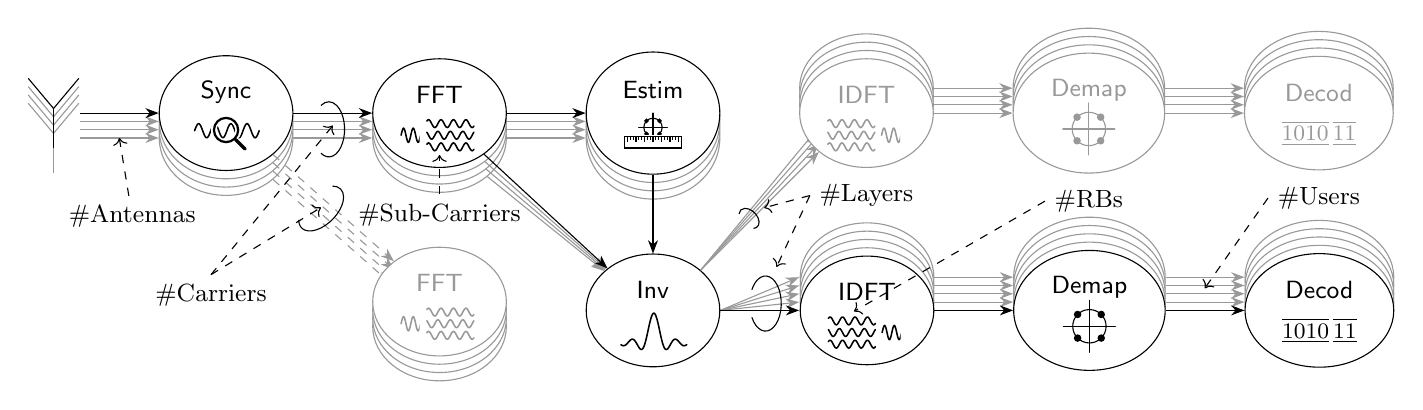
\begin{tikzpicture}

	\draw [yshift=0] pic (A3) {frontend=gray!80};
	\draw [yshift=3] pic (A2) {frontend=gray!80};
	\draw [yshift=6] pic (A1) {frontend=gray!80};
	\draw [yshift=9]  pic (A0) {frontend=black};
	
	
	\node at (1,-1) (antLabel) {\lblTextsize\#Antennas};
	\node at (2,-2) (carrierLabel) {\lblTextsize\#Carriers};
	\node at ($(A0-c.south)!0.6!(A0-d.north)$) (scCnt) {\lblTextsize\#Sub-Carriers};
	
	\draw [->, dashed] (antLabel)  -- ($(A3-ant.east)!0.5!(A3-b.west)$);
	\draw [->, dashed] (carrierLabel.north)  -- ($(A0-b.east)!0.5!(A3-c.west)$);
	\draw [->, dashed] (carrierLabel.north)  -- ($(A0-b.south east)!0.4!(A3-d.north west)$);
	\draw [->, dashed] (scCnt.north)  -- ++(90:0.5cm);
	
	\node[blub=black, below= of A0-e] (B) {
		\tikz{ 
			\pic [anchor=center] at (0,0) {equalizer};
		}
	};

	\foreach \y in {4,3,...,1}{
		\pgfmathparse{\y*3}
		\edef\yStart{\pgfmathresult}
		\node[yshift=\yStart, right= of B, inner sep=0] (C\y) {
			\tikz{ 
				\pic [inner sep=0, anchor=center] at (0,0) {backend=gray!80};
			}
		};
		\draw [gray!80, -Stealth] (B.east) -- (C\y.west);
	}

	\node[right= of B, inner sep=0] (C) {
		\tikz{ 
			\pic [inner sep=0, anchor=center] {backend=black};
		}
	};

	\foreach \y in {3,2,1}{
		\pgfmathparse{\y*3}
		\edef\yStart{\pgfmathresult}
%		\node[yshift=\yStart, above= of C, align=center, inner sep=0] (C_\y) {
%			\tikz{ 
%				\pic [inner sep=0, anchor=center] at (0,0) {backend=gray!80};
%			}
%		};
	
		\draw  pic [anchor=west] (C_\y) at ([yshift=\yStart] C.west |- A0-e.east) {backend=gray!80};
		\draw [gray!80, -Stealth] (B.north east) -- (C_\y-a.south west);
	}


	\draw  pic [anchor=west] (C_0) at (C.west |- A0-e.east) {backend=gray!80};
	\draw [gray!80, -Stealth] (B.north east) -- (C_0-a.south west);
	
	\node at ([yshift=-0.35cm]C_0-a.south) (layerCnt) {\lblTextsize\#Layers};
	\node at ([yshift=-0.35cm]C_0-b.south) (rbCnt) {\lblTextsize\#RBs};
	\node at ([yshift=-0.35cm]C_0-c.south) (userCnt) {\lblTextsize\#Users};
	
	\draw [->, dashed] (rbCnt.west) -- ++(210:2.8cm);
	\draw [->, dashed] (userCnt.west) -- ++(235:1.4cm);
	\draw [->, dashed] (layerCnt.west) -- ++(195:0.6cm);
	\draw [->, dashed] (layerCnt.west) -- ++(245:1cm);


	\draw [-Stealth] (A0-e) -- (B);
	\draw [-Stealth, gray!80] (A1-c) -- (B);
	\draw [-Stealth, gray!80] (A2-c) -- (B);
	\draw [-Stealth, gray!80] (A3-c) -- (B);
	\draw [-Stealth] (A0-c) -- (B);
	
	\draw [-Stealth] (B) -- (C);
	
	\draw  ($ (A0-b.south east)!0.4!(A0-c.south west) $ ) arc(-120:120:0.2 and 0.35);
	\draw  [rotate=-45] ([shift=(-90:0.4cm)]$ (A0-b.south east)!0.4!(A0-d.north west) $ ) arc(-120:120:0.2 and 0.35);

	\draw  ([yshift=-2.5]$ (B.east)!0.4!(C.west) $ ) arc(-150:150:0.2 and 0.35);
	\draw  [rotate=45] ([shift=(90:-0.1cm)]$ (B.north east)!0.4!(C_0-a.south west) $ ) arc(-120:120:0.1 and 0.15);


%	\coordinate (origin) at (0,0);
%	\coordinate (xmax) at ([xshift=8.5cm] origin);
%	\coordinate (ymax) at ([yshift=3.8cm] origin);
%	\coordinate (y1) at ([yshift=2.5cm] origin);
%	
%	\foreach \x/\xl in {0/, 1/0.1M, 2/1M/, 3/10M, 4/100M, 5/1G, 6/10G, 7/100G, 8/1T}
%	\draw (\x,0.0) -- (\x,-0.1) node [below] {\xl};
%	\foreach \y/\yl in {0/1000, 1/100, 2/10, 3/1}
%	\draw (0.0,\y) -- (-0.1,\y) node [left] {\yl};
%	
%	\draw [->, very thick] (origin) -- (xmax) node [midway, below, yshift=-15](xlabel) {Throughput [bps]};
%	\draw [->, very thick] (origin) -- (ymax) node [midway, left, xshift=-20, rotate=90, anchor=south](ylabel) {Latency [ms]};
%
%	\draw [rounded corners, fill=gray!5, name path=6G] (0,0) rectangle (8,3.2) node[below left=]{6G};
%	\draw [rounded corners, fill=gray!10, name path=5G] (0,0) rectangle (6,2.4) node[below left=]{5G};
%	\draw [rounded corners, fill=gray!15, name path=4G] (0,0) rectangle (4.5,1.3) node[below left=]{4G};
%	\draw [rounded corners, fill=gray!80, name path=3G] (0,0) rectangle (3.1,1) node[below left=]{3G};
%	\draw [rounded corners, fill=gray!25, name path=2G] (0,0) rectangle (1.3,1) node[below left=]{2G};
%	
%	\draw [Stealth-Stealth, red, ultra thick] (0.3,0.25cm) -- ++ (7.7cm,0)
%		node [very near end, above]{$\sim 10^7$};
%	\draw [Stealth-Stealth, red, ultra thick] (0.25,0.3cm) -- ++ (0, 2.9cm)
%	node [very near end, right]{$\sim 10^3$};
%	
	
\end{tikzpicture}